\begin{frame}{(Continuous) Integration of scientific software} 
    \framesubtitle{Hands on: creating a Docker image} 

    \vfill

    In the \textbf{\texttt{minimal-cse-ci-examples}} repository


    \mint{bash}+?> git checkout starting-point+
    \mint{bash}+?> git checkout -b feature/dockerfile+

\end{frame}

\begin{frame}{(Continuous) Integration of scientific software} 
    \framesubtitle{Hands on: creating a Docker image I} 
    \vfill

    \begin{columns}
        \begin{column}[c]{0.5\textwidth}
            \centering
            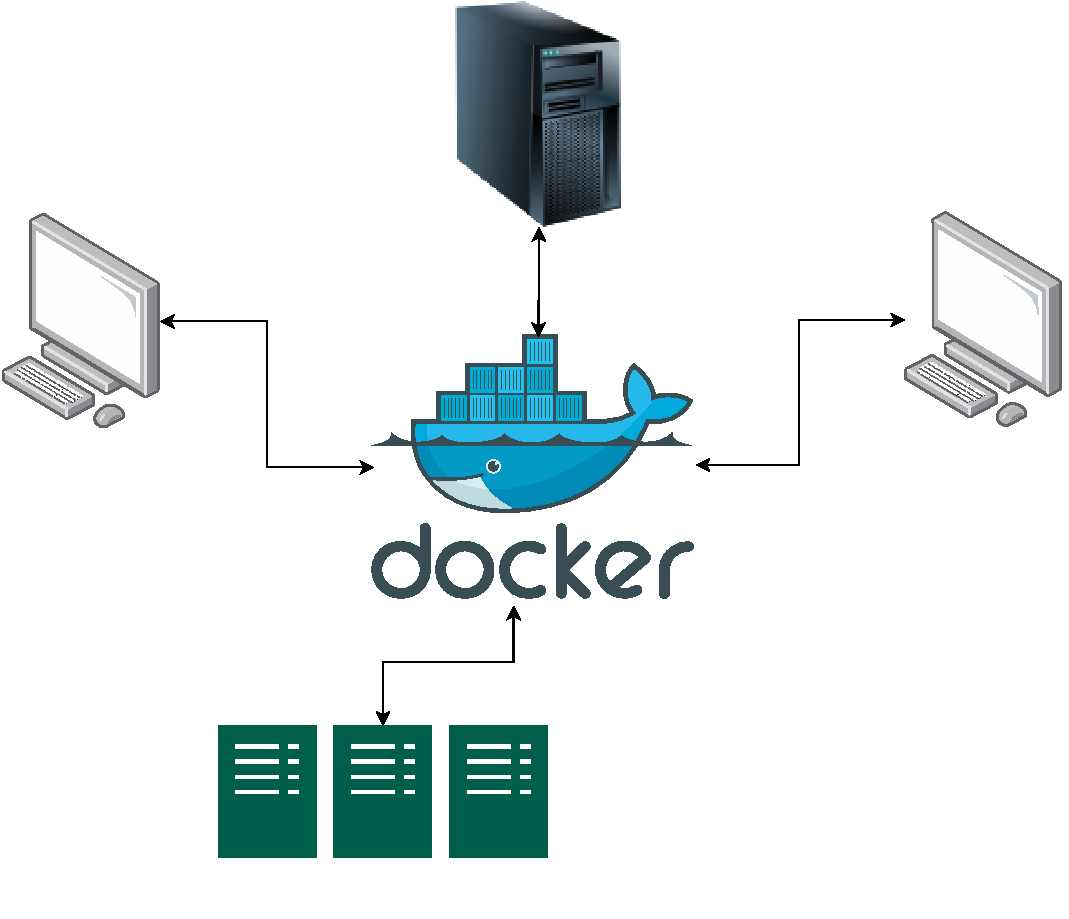
\includegraphics[width=0.8\columnwidth]{figures/docker-description.pdf}
        \end{column}
        \begin{column}[c]{0.5\textwidth}

            \begin{itemize}
                \item \href{https://docs.docker.com/}{Docker} images are computing environments that contain (\textbf{dependencies}) needed to build the research software, run simulations and process results. 
                \item Sharing docker images removes the need to install the dependencies on different machines. 
                \item The computing environment in a Docker image is usually based on an existing Linux distribution. 
                \item The Docker image is built from a text file, that specifies installation steps for the dependencies, the so-called \textbf{Dockerfile}.
            \end{itemize}
        \end{column}
    \end{columns}
\end{frame}

\begin{frame}[fragile]{(Continuous) Integration of scientific software} 
    \framesubtitle{Hands on: creating a Docker image II} 
    \vfill

    In a file named 'minimal-cse-ci-dockerfile\_ubuntu-focal', write \\

    \begin{minted}{docker}
FROM ubuntu:focal 

# Set timezone
RUN apt-get update --fix-missing && \
    DEBIAN_FRONTEND="noninteractive" apt-get -y install tzdata
    \end{minted}

    \begin{itemize}
        \item We'll use Ubuntu 20.04 (focal) as the base system.
        \item Steps that are usually done manually (setting the timezone) are automated. 
    \end{itemize}

\end{frame}

\begin{frame}[fragile]{(Continuous) Integration of scientific software} 
    \framesubtitle{Hands on: creating a Docker image III} 
    \vfill

    Dependency installation 

    \begin{columns}
        \begin{column}[c]{0.5\textwidth}
    \begin{minted}[fontsize=\footnotesize]{docker}
# Install packages
RUN apt update && apt-get install --fix-missing -y \
    # Building
    build-essential cmake \
    # Version control
    git \
    # Python
    python3 \ 
    # Visualization
    python3-matplotlib python3-numpy \
    # Data analysis
    python3-pandas \
    # Test visualization
    jupyter-notebook jupyter-nbconvert \
    # Debugging the image 
    vim  
    \end{minted}
        \end{column}
        \begin{column}[c]{0.5\textwidth}
            \begin{itemize}
                \item \textbf{RUN} runs commands in the \textbf{Docker container}. 
                \item The \textbf{Docker container} is a process spawned using the Docker image as the computing environment.
                \item Install the software needed for the scientific workflow (dependencies).
            \end{itemize}
        \end{column}
    \end{columns}


\end{frame}

\begin{frame}[fragile]{(Continuous) Integration of scientific software} 
    \framesubtitle{Hands on: creating a Docker image IV} 
    \vfill

    Software setup  

    \begin{minted}{docker}
## Default Ubuntu to python3
RUN update-alternatives --install \
    /usr/bin/python python /usr/bin/python3 10 
    \end{minted}

    \medskip

    Some specifics

    \begin{itemize}
        \item Alternative (\textbf{g++}) compiler. 
        \item Alternative working directory. 
    \end{itemize}

\end{frame}

\begin{frame}[fragile]{(Continuous) Integration of scientific software} 
    \framesubtitle{Hands on: creating a Docker image V} 
    \vfill
    \begin{columns}
        \begin{column}[c]{0.5\textwidth}
    \noindent{\scriptsize\href{https://gitlab.com/tmaric/minimal-cse-ci-examples/-/blob/main/minimal-cse-ci-dockerfile_ubuntu-focal}{Complete Dockerfile for the minimal example}}
    \begin{minted}[fontsize=\tiny]{docker}
FROM ubuntu:focal 

# Set timezone
RUN apt-get update --fix-missing && \
    DEBIAN_FRONTEND="noninteractive" apt-get -y install tzdata

# Install packages
RUN apt update && apt-get install --fix-missing -y \
    # Building
    build-essential cmake \
    # Version control
    git \
    # Python
    python3 \ 
    # Visualization
    python3-matplotlib python3-numpy \
    # Data analysis
    python3-pandas \
    # Test visualization
    jupyter-notebook jupyter-nbconvert \
    # Debugging the image 
    vim  

## Default Ubuntu to python3
RUN update-alternatives --install \
    /usr/bin/python python /usr/bin/python3 10 
    \end{minted}
        \end{column}
        \begin{column}[c]{0.5\textwidth}
            \begin{itemize}
                \item The example Dockerfile installs all dependencies for the minimal example on Ubuntu 20.04.
                \item The installation commands would be different for another operating system.  
                \item A more complex software (e.g. OpenFOAM) requires a larger Dockerfile.
                \item This lets us define the computing environments that are supported by the research software. 
            \end{itemize}
        \end{column}
    \end{columns}
\end{frame}

\begin{frame}[fragile]{(Continuous) Integration of scientific software} 
    \framesubtitle{Hands on: creating a Docker image VI} 
    \vfill

    Building the image

\begin{minted}{shell}
%?> sudo docker build . \
    %-f minimal-cse-ci-dockerfile_ubuntu-focal \
    %-t minimal-cse-ci-dockerfile_ubuntu-focal
    sudo docker build . -f minimal-cse-ci-dockerfile_ubuntu-focal -t minimal-cse-ci:ubuntu-focal
\end{minted}

\begin{itemize}
    \item "\texttt{.}": current directory
    \item "-f" name of the Dockerfile (defaults to "Dockerfile")
    \item "-t" tag (name) of the Docker image
\end{itemize}

\end{frame}

\begin{frame}[fragile]{(Continuous) Integration of scientific software} 
    \framesubtitle{Hands on: creating a Docker image VII} 
    \vfill

    Listing Docker images

    \begin{minted}[fontsize=\footnotesize]{bash}
?> sudo docker image list
REPOSITORY                             TAG    IMAGE   ID   CREATED        SIZE
minimal-cse-ci-dockerfile_ubuntu-focal latest 921233ec4b44 9 minutes ago 982MB
    \end{minted}

    \begin{itemize}
        \item The image is built on the machine (host) where the \textbf{\texttt{docker build}} command is called. 
        \item Docker uses a so-called \textbf{image registry} to store images.
        \item For Continuous Integration the images are built on the machine where the tests are run or shared on \href{https://hub.docker.com/}{\textbf{Dockerhub}}.
    \end{itemize}

\end{frame}

\begin{frame}[fragile]{(Continuous) Integration of scientific software} 
    \framesubtitle{Hands on: creating a Docker image VIII} 
    \vfill

    "\textbf{Spinning a container}" (running a Docker image) 

    \begin{minted}{bash}
?> sudo docker run -it minimal-cse-ci-dockerfile_ubuntu-focal /bin/bash
root@b2c14ee0fd58:/# ls
bin  boot  dev  etc  home  lib  lib32  lib64  libx32  media  mnt  
opt  proc  root  run  sbin  srv  sys  tmp  usr  var
root@b2c14ee0fd58:/# cd 
root@b2c14ee0fd58:~# pwd
/root
    \end{minted}

    \begin{itemize}
        \item The container behaves just like a "regular" Ubuntu. 
        \item \textbf{Jobs (test) commands for the Continuous Integration are checked/debugged inside a running container.}
            \begin{itemize}
                \item Forgot to install a dependency.
                \item The research software does not compile with installed dependencies.
                \item ...
            \end{itemize}
    \end{itemize}

\end{frame}


\begin{frame}[fragile]{(Continuous) Integration of scientific software} 
    \framesubtitle{Hands on: creating a Docker image IX} 
    \vfill

    Working within the container : compiling the software

    \begin{minted}{bash}
?> git clone https://gitlab.com/tmaric/minimal-cse-ci-examples.git
?> cd minimal-cse-ci-examples && mkdir build && cd build
?> cmake .. && make
?> ./myapp
    \end{minted}

    The same steps will be done in the Docker container by the Continuous Integration  
    \begin{itemize}
        \item Clone the repo. 
        \item Build the software.  
        \item Run the tests. 
    \end{itemize}

\end{frame}


\begin{frame}[fragile]{(Continuous) Integration of scientific software} 
    \framesubtitle{Hands on: creating a Docker image X} 
    \vfill

    Analyzing the data using Jupyter notebooks

\begin{minted}{bash}
   ?> cd ..
   ?> jupyter nbconvert --execute mynotebook.ipynb --to html 
\end{minted}

    \begin{itemize}
        \item On the cluster, one would start the Jupyter notebook server and connect to it locally. 
        \item Here the notebook is used to process the results and visualize secondary data as tables and diagrams.
    \end{itemize}

\end{frame}

\begin{frame}[fragile]{(Continuous) Integration of scientific software} 
    \framesubtitle{Hands on: creating a Docker image XI} 
    \vfill

    Extracting the data from the container:
    \begin{itemize}
        \item Find the ID of the container you're on (execute on your machine)
            
            \begin{minted}{bash}
sudo docker ps 
            \end{minted}

        \item Copy the results from the container onto the local machine (execute on your machine)
            \begin{minted}{bash}
mkdir container-data
sudo docker cp f2dff55edf7a:/root/minimal-cse-ci-examples \
    container-data/
            \end{minted}
        \item Examine the data and the Jupyter notebook in a browser.
    \end{itemize}

    Note: the sequence f2dff55edf7a is system dependent ID, so it'll be different for you.

\end{frame}

\begin{frame}[fragile]{(Continuous) Integration of scientific software} 
    \framesubtitle{Hands on: creating a Docker image XII} 
    \vfill

    \begin{itemize}
        \item Saving the container or an image as a tar file 

    \begin{minted}{bash}
sudo docker commit f2dff55edf7a test:latest
    \end{minted}

        \item You can exit/close the container by pressing Ctrl+d.

        \item View the newly create image with 'name:tag' using 

    \begin{minted}{bash}
sudo docker image list 

REPOSITORY TAG     IMAGE ID       CREATED              SIZE
test       latest  f2dff55edf7a   About a minute ago   983MB
    \end{minted}

    \item Save the image into a tar file 

    \begin{minted}{bash}
sudo docker save test:latest -o container-archive.tar
    \end{minted}

    \item Load an image into Docker's registry to work with it 

    \begin{minted}{bash}
    sudo docker load -i container-archive.tar
    \end{minted}

\end{itemize}

\end{frame}


\begin{frame}[fragile]{(Continuous) Integration of scientific software} 
    \framesubtitle{Hands on: creating a Docker image XIII} 
    \vfill

    \begin{itemize}
        \item Usually, the Docker image "lives" locally on the test machine. 
        \item However, it can also be shared publicly on Dockerhub, for example (don't do this now)

            \begin{minted}{docker}
                ?> docker login 
                ?> docker tag name:tag username/name:tag
                ?> docker push username/name:tag
            \end{minted}
        \item This image can now be used by everyone.
        \item Note: once you exit/stop a container all data/files created inside the container are discarded. 

    \end{itemize}

\end{frame}

\begin{frame}{(Continuous) Integration of scientific software} 
    \framesubtitle{Hands on: creating a Docker image XIV} 
    \vfill

    \begin{columns}
        \begin{column}[c]{0.55\textwidth}
            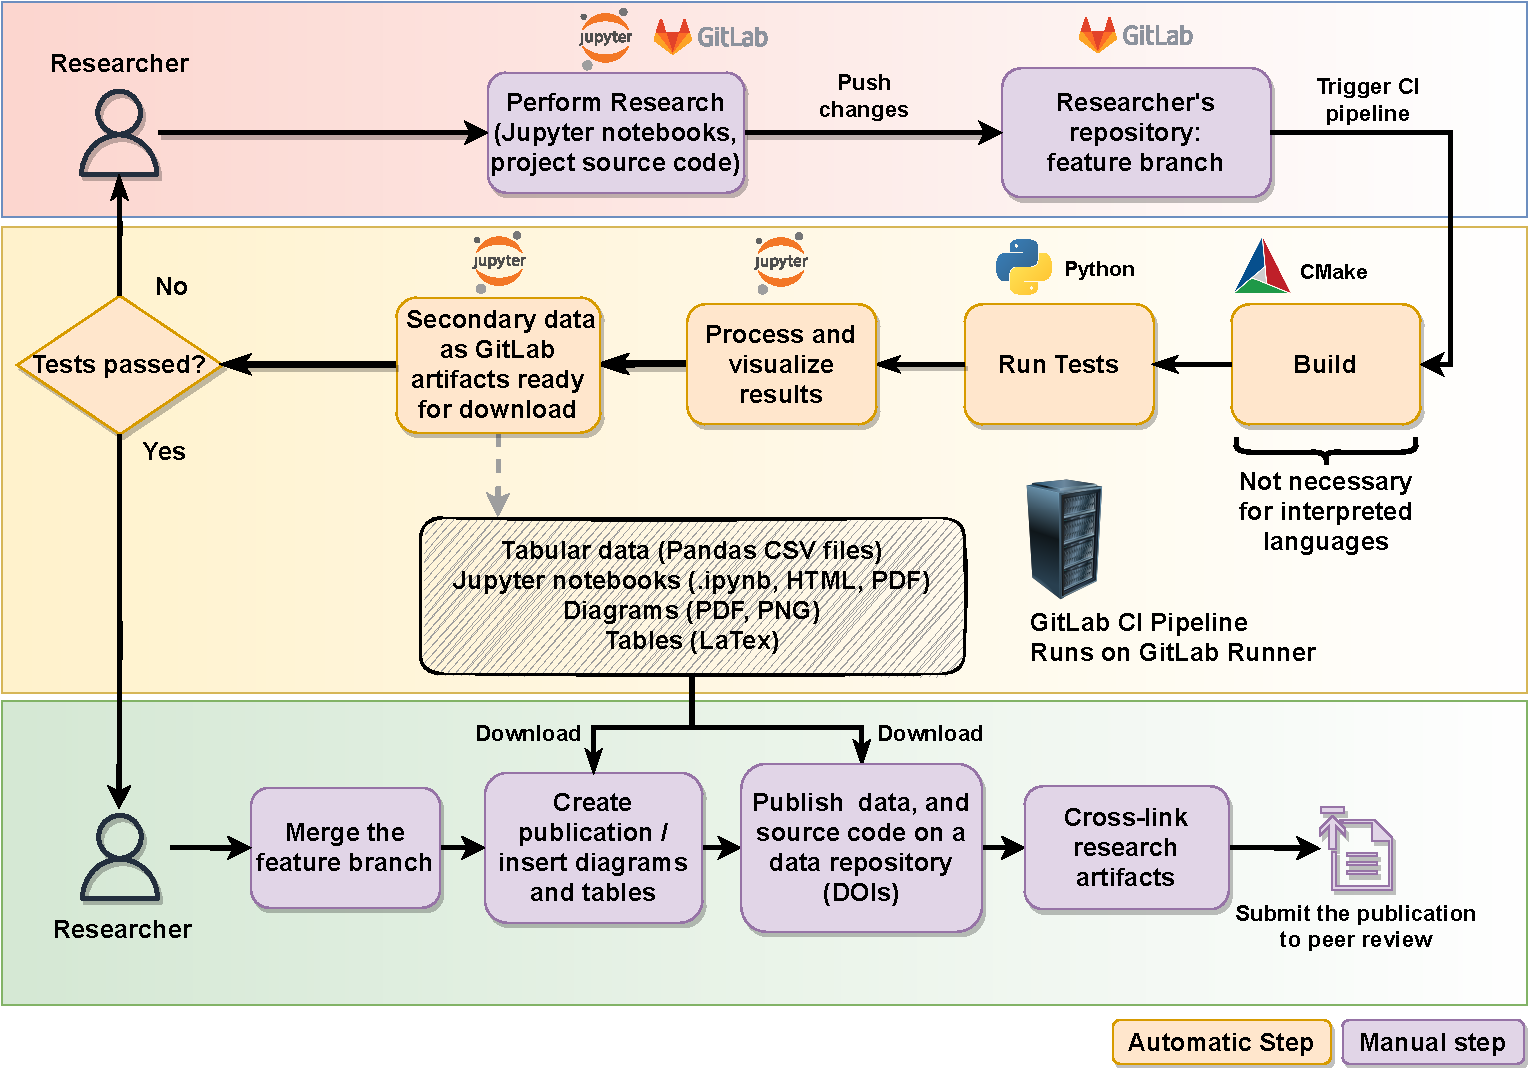
\includegraphics[width=\columnwidth]{figures/ZINF-CI-diagram-individual.pdf}
        \end{column}
        \begin{column}[c]{0.40\textwidth}
            All the steps done so far manually using Docker, namely,

            \begin{enumerate}
                \item \textbf{building} the scientific software, 
                \item \textbf{running tests}, 
                \item \textbf{processing data} 
                \item \textbf{exporting} the data and Jupyter notebooks, 
            \end{enumerate}

            are automated by Continuous Integration, that uses Docker for encapsulating the computing environment. 
        \end{column}
    \end{columns}

\end{frame}

%\begin{frame}[fragile]{(Continuous) Integration of scientific software} 
    %\framesubtitle{Hands on: creating a Docker image II} 
    %\vfill

    %\begin{itemize}
        %\item The .tar file can be used to store the research software, its computing environment and all the results from a publication. 

        %\item Unfortunately, root privileges are required. 

        %\item This complicates the use of Docker on HPC Clusters, and data reproduction without root-rights. 

        %\item Check out \href{

    %\end{itemize}

%\end{frame}

